%for a more compact document, add the option openany to avoid
%starting all chapters on odd numbered pages
\documentclass[12pt]{cmuthesis}

% This is a template for a CMU thesis.  It is 18 pages without any content :-)
% The source for this is pulled from a variety of sources and people.
% Here's a partial list of people who may or may have not contributed:
%
%        bnoble   = Brian Noble
%        caruana  = Rich Caruana
%        colohan  = Chris Colohan
%        jab      = Justin Boyan
%        josullvn = Joseph O'Sullivan
%        jrs      = Jonathan Shewchuk
%        kosak    = Corey Kosak
%        mjz      = Matt Zekauskas (mattz@cs)
%        pdinda   = Peter Dinda
%        pfr      = Patrick Riley
%        dkoes = David Koes (me)

% My main contribution is putting everything into a single class files and small
% template since I prefer this to some complicated sprawling directory tree with
% makefiles.

% some useful packages
\usepackage{times}
\usepackage{fullpage}
\usepackage{graphicx}
\usepackage{amsmath}
\usepackage{cite}
\usepackage[numbers,sort]{natbib}
\usepackage[pageanchor=true,plainpages=false, pdfpagelabels, bookmarks,bookmarksnumbered,
%pdfborder=0 0 0,  %removes outlines around hyper links in online display
]{hyperref}
\usepackage{setspace}
\usepackage{subfigure}
\usepackage{titlesec}
\titleformat{\chapter}[hang] 
{\normalfont\LARGE\bfseries}{\chaptertitlename\ \thechapter:}{1em}{}

% Approximately 1" margins, more space on binding side
%\usepackage[letterpaper,twoside,vscale=.8,hscale=.75,nomarginpar]{geometry}
%for general printing (not binding)
\usepackage[letterpaper,twoside,vscale=.8,hscale=.75,nomarginpar,hmarginratio=1:1]{geometry}

% Provides a draft mark at the top of the document. 
\draftstamp{\today}{DRAFT}

\begin {document} 
\frontmatter

%initialize page style, so contents come out right (see bot) -mjz
\pagestyle{empty}

\title{ %% {\it \huge Thesis Proposal}\\
{\bf PROPOSAL: Unsupervised Guitar String Classification for Tablature Transcription}}
\author{Jonathan Michelson}
\date{April 2017}
\Year{2017}
\trnumber{}

\committee{
Professor Richard Stern \\
Professor Tom Sullivan \\
}

\support{}
\disclaimer{}

% copyright notice generated automatically from Year and author.
% permission added if \permission{} given.

%\keywords{Stuff, More Stuff}

\maketitle

%\begin{dedication}
%For my dog
%\end{dedication}

\pagestyle{plain} % for toc, was empty

%% Obviously, it's probably a good idea to break the various sections of your thesis
%% into different files and input them into this file...

%\doublespacing
%\begin{abstract}
%Guitar tablature transcription (brief explanation) is a commonly used music notation standard that could benefit from automation. Previous work solves this task in a framework that requires prior information about the guitar. Here, an unsupervised offline solution is introduced. Inharmonicity estimates extracted from isolated guitar notes naturally segregate into semi-linear formations determined by its sourced string. The inharmonicities are modeled with a linear regression mixture, and optimized with expectation maximization. 
%\end{abstract}
%\singlespacing

%\begin{acknowledgments}
%My advisor is cool.
%\end{acknowledgments}



%\tableofcontents
%\listoffigures
%\listoftables

\mainmatter

%% Double space document for easy review:
%\renewcommand{\baselinestretch}{1.66}\normalsize

% The other requirements Catherine has:
%
%  - avoid large margins.  She wants the thesis to use fewer pages, 
%    especially if it requires colour printing.
%
%  - The thesis should be formatted for double-sided printing.  This
%    means that all chapters, acknowledgements, table of contents, etc.
%    should start on odd numbered (right facing) pages.
%
%  - You need to use the department standard tech report title page.  I
%    have tried to ensure that the title page here conforms to this
%    standard.
%
%  - Use a nice serif font, such as Times Roman.  Sans serif looks bad.
%
% Other than that, just make it look good...
\chapter{Proposal}
\noindent
\textbf{Background} - The guitar is a widely popular musical instrument. Because the pitch ranges of its adjacent strings overlap, a given musical phrase can usually be realized in a few different ways. Conventional music scores represent passages as notes and chords, and therefore leave fretboard position ambiguous. Tablature is an alternative music notation for guitarists that doesn't suffer from the one-to-many mapping of scores. Automating its tedious annotation process is an interesting MIR problem that has applications in music education and research.

\noindent
\textbf{Previous Work} - String separation for violin audio recordings is discussed in~\cite{maezawa2009}. Guitar tablature transcription with a hexaphonic pickup is presented in~\cite{ogrady2009}. Signal processing-based solutions for guitar string transcription can be found in ~\cite{barbanchoa2012,barbanchoi2012}. Machine learning approaches~\cite{barbancho2009, abesser2012, kehling2014} show success.

\noindent
\textbf{Missing Science} - The previous work generally focused on solutions which required prior or typically unavailable information. In~\cite{ogrady2009}, access to an uncommon and potentially hindering hexaphonic pickup is required. In signal processing approaches like ~\cite{barbanchoi2012}, "seeding" the system with known open strings is necessary. In supervised machine learning approaches like ~\cite{abesser2012, kehling2014}, the classifier must be trained with labeled guitar notes. This has the additional drawback of restricting success to guitars tuned identically to those of the test set. In other ML approaches~\cite{barbancho2009}, the guitar audio is generated from only standard chord positions. 

\noindent
\textbf{Proposed Solution} -  We estimate clean, isolated, monophonic, electric guitar notes' inharmonicities, plot them vs $f_0$, and fit them with a linear regression mixture model~\cite{faria2010}. We assign clusters (string identities) based on the converged mixture model. This doesn't require prior information like string tuning or labeled training instances. However if tuning information is supplied by the user, we can trivially infer the tablature (string-fret labels) of each note.

\noindent
\textbf{Pilot Results} - Figure \ref{fig:beta} shows best-case results for inharmonicity estimation and plotting. In Figure \ref{fig:em}, current best-case results for linear regression estimation are shown. Classification F-scores by string are $[1.0, 1.0, 0.89, 0.8, 0.57, 1.0]$. Average F-score $ = 0.88$.

\begin{figure}[h]
\centering
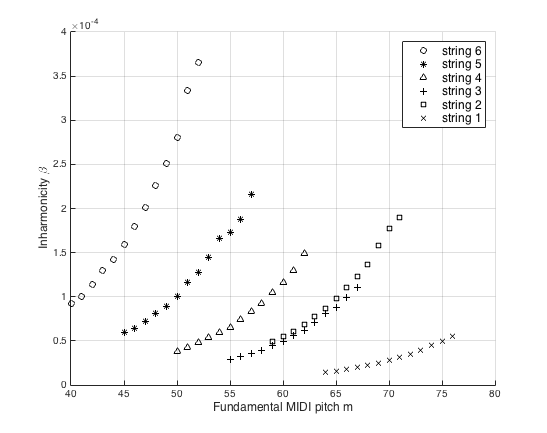
\includegraphics[scale=.6]{beta-v-midi.png}
\caption{Inharmonicities $\beta$ (y-axis) vs. MIDI note number (x-axis). The six different colors correspond to the six string labels E2, A2, D3, G3, B3, E4. This electric guitar recording enumerated the 78 notes between E2 and E5 inclusive in standard-tuning.}
\label{fig:beta}
\end{figure}

\begin{figure}[h]
\centering
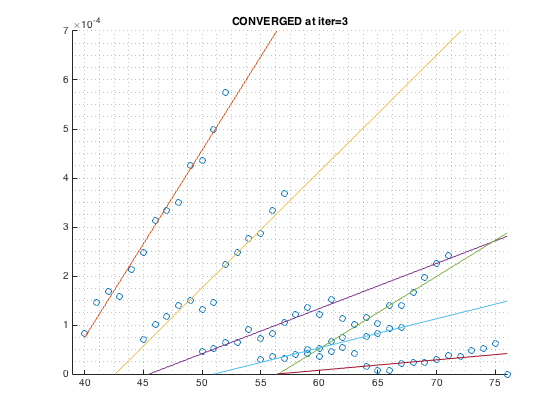
\includegraphics[scale=0.6]{em.png}
\caption{Converged EM estimate of the linear regressions. Same axes as fig. \ref{fig:beta}.}
\label{fig:em}
\end{figure}

\noindent
\textbf{Work to be Done} - Our EM implementation still needs to: (1) estimate the optimal number of mixtures $J$ on its own; (2) initialize mixture centers (regression weight vectors) on its own; (3) address a singularity bug (variance goes to 0, likelihood goes to $\infty$); (4) incorporate a formal classification step. We also need to (5) conduct experiments over full electric guitar dataset.

\noindent
\textbf{Evaluation Criteria}
String classification F-scores to evaluate mixture model accuracy for training set. For unlabeled test data, various cluster analytics to obtain "optimal" clustering.

\noindent
\textbf{Deliverables} - Proposal (draft + final); thesis (draft + final).

\noindent
\textbf{Timetable} - Proposal draft: 3/29; proposal final: 4/1; thesis draft: 4/24; thesis final: 5/1.

%\appendix
%\include{appendix}

\backmatter

%\renewcommand{\baselinestretch}{1.0}\normalsize

% By default \bibsection is \chapter*, but we really want this to show
% up in the table of contents and pdf bookmarks.
\renewcommand{\bibsection}{\chapter{\bibname}}
%\newcommand{\bibpreamble}{This text goes between the ``Bibliography'' header and the actual list of references}
\bibliography{mybib} %your bib file
\bibliographystyle{plainnat}


\end{document}
